\documentclass[12pt]{article}
\usepackage[utf8]{inputenc}
\usepackage{pgf,tikz,pgfplots}
\pgfplotsset{compat=1.15}
\usepackage{mathrsfs}
\usetikzlibrary{arrows}
\usepackage{fontspec}
\setmainfont[Renderer=ICU,Mapping=tex-text]{Cousine}
\usepackage{amssymb}
\usepackage[paperwidth=8.2cm,paperheight=20.7cm,left=0.1cm,right=0.1cm,top=0.1cm,bottom=0.1cm]{geometry}
\begin{document}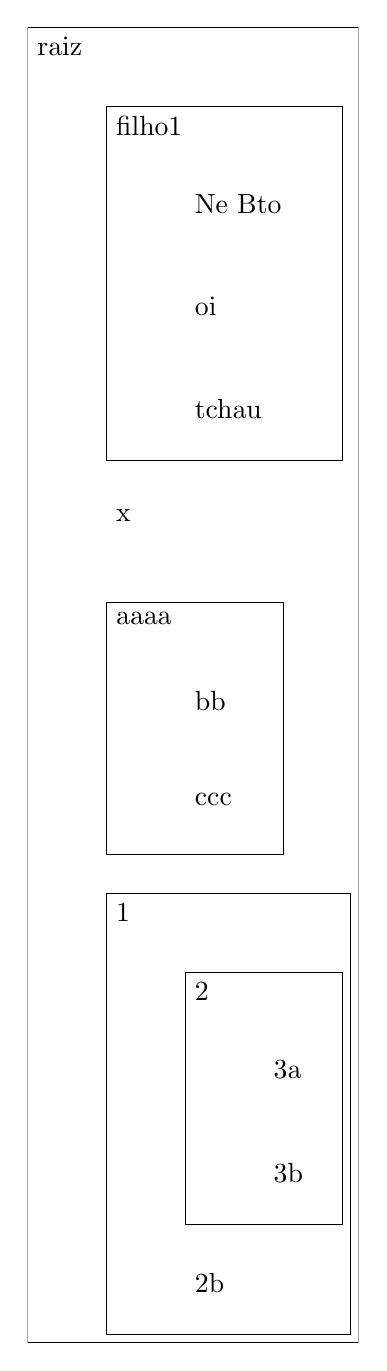
\begin{tikzpicture}[line cap=round,line join=round,>=triangle 45,x=1cm,y=1cm]
\clip(0, 0)rectangle(4.199999999999999, -16.7);

\draw(0, 0) node[anchor=north west] {raiz};
\draw (0, 0) rectangle (4.199999999999999,-16.7);
\draw(1, -1) node[anchor=north west] {filho1};
\draw (1, -1) rectangle (4.0,-5.499999999999999);
\draw(2, -2) node[anchor=north west] {Ne Bto};

\draw(2, -3.3) node[anchor=north west] {oi};

\draw(2, -4.6) node[anchor=north west] {tchau};

\draw(1, -5.999999999999999) node[anchor=north west] {x};

\draw(1, -7.299999999999999) node[anchor=north west] {aaaa};
\draw (1, -7.299999999999999) rectangle (3.2500000000000004,-10.499999999999998);
\draw(2, -8.299999999999999) node[anchor=north west] {bb};

\draw(2, -9.599999999999998) node[anchor=north west] {ccc};

\draw(1, -10.999999999999998) node[anchor=north west] {1};
\draw (1, -10.999999999999998) rectangle (4.1,-16.599999999999998);
\draw(2, -11.999999999999998) node[anchor=north west] {2};
\draw (2, -11.999999999999998) rectangle (4.0,-15.199999999999998);
\draw(3, -12.999999999999998) node[anchor=north west] {3a};

\draw(3, -14.299999999999997) node[anchor=north west] {3b};

\draw(2, -15.699999999999998) node[anchor=north west] {2b};

\end{tikzpicture}

\end{document}